\section{Aikaisempi tutkimus}
% \section{Background}

Tässä osassa selvitetään, mitä tutkimuksen kohteena olevasta aiheesta tiedetään
entuudestaan. Selvityksen tulee kattaa tasapainoisesti koko tutkimuskenttä. 

Kun opinnäytetyötä kirjoitetaan, on noudatettava ohjeita, jotka koskevat
opinnäytteen rakennetta, käytäntöjä, muotoseikkoja sekä ulkoasua. Esitellään
näitä ohjeita tarkemmin.

%% Osan hienojaottelua alaosiin, eikä välttämättä edes tarpeen, tässä vain
%% esimerkkinä. Käytä harkintasi mukaan osan jaottelua, joskus alaotsikot
%% selventävät asioita ja joskus vain sirpaloittavat tarpeettomasti tekstiä.
%%  Jaottelu menee seuraavasti:
%% \section{osan otsikko} 
%% \subsection{alaotsikko}
%% \subsubsection{ala-alaotsikko}
%% Tätä pitemälle ei pidä jaotella. 

\subsection{Rakenne}

Opinnäytteen rakenteen tulee olla hyvän tieteellisen kirjoittamisen käytännön
mukainen ja sisältää vähintään seuraavat osat:

\begin{enumerate}
\item Nimiölehti
\item Tiivistelmä
\item Sisällysluettelo
\item Symboli- ja lyhenneluettelo (ei yleensä käytetä systiksen kanditöissä)
\item \label{a} Johdanto
%% Tässä alla on esimerkki lainausmerkkien käytöstä. Suomalaisen tekstin
%% lainausmerkit eivät mene oikein latexissa (tai monissa muissakaan
%% julkaisujärjestelmissä) kun käytetään "-merkkiä, koska latex käyttää
%% amerikkalaista lainausmerkkien tulostustapaa. Vaihtoehtona voi käyttää
%% kulmalainausmerkkejä, jotka myös tulostuvat oikein.
\item  Aikaisempi tutkimus. Työn luonteen niin vaatiessa otsikko voi olla myös
        >>Teoreettinen tausta>>  tai näiden otsikoiden yhdistelmä.
\item Tutkimusaineisto ja -menetelmät. Otsikko voi olla myös jotain muuta, jos se sopii paremmin työn luonteeseen. %% yhdysmerkki - eli tavuviiva. 
\item Tulokset
\item \label{o} Tarkastelu. Työn luonteen niin vaatiessa otsikko voi olla myös
		>>Johtopäätökset>> tai >>Yhteenveto>> tai edellä mainittujen otsikoiden
		yhdistelmä.
\item Lähteet
\item Liitteet.
\end{enumerate}

Tiivistelmän ja symboli- sekä lyhenneluetteloiden väliin voi sijoittaa
halutessaan esipuheen.  

Työn osat \ref{a}--\ref{o} muodostavat \textit{tekstiosan.}  Työn yksittäisiä
osia voidaan jakaa alaotsikoilla alaosiin, joita ei ole yllä esitetty. 
Alaotsikoiden käyttäminen selventää parhaimmillaan tekstiä, ja pahimmillaan 
sirpaloittaa sitä.  Sirpaloitumista voi estää huolehtimalla siitä, että samalla 
sivulla ei esiinny useampaa alaotsikkoa. Tekstin jäsentelyssä on yleensä 
ongelmia, jos osassa on vain yksi alaosa, tai kirjoittaja joutuu käyttämään 
useampaa kuin kahta tasoa (osa ja alaosat): alaosien alaosat ovat harvoin tarpeen.

\subsection{Sivut ja kirjaintyypit}

Opinnäytteen tulee olla kirjoitettu koneella tai
tekstinkäsittelyohjelmalla yksipuolisesti A4-kokoiselle paperille.
Kandidaatintyön tekstiosan sopiva pituus on noin 15--20 sivua ja
diplomityön noin 60 sivua. Työtä ei ole syytä tarpeettomasti pidentää.

Opinnäytteen tekstiosan kirjaintyypin tulee olla antiikva eli
%% esimerkki pakkotavutuksesta; "serif-tyyppinen" on tavutuksen kannalta
%% hankala, joten pakkotavutetaan se. 
serif\--tyyp\-pi\-nen ja lisäksi kursivoimaton, lihavoimaton sekä kooltaan 12
pistettä (kuten tässä esityksessä). Groteskeja eli \textsf{Sans serif}-tyyppisiä
kirjaintyyppejä (kuten Helvetica tai Arial) ei saa käyttää varsinaisessa
tekstissä, mutta otsikoissa näitä voidaan käyttää.  Otsikoissa voidaan käyttää
kooltaan edellä mainittua suurempaa kirjaintyyppiä sekä tyylikeinoja, kuten
lihavointia tai kursivointia. Tekstissä samantasoisten otsikoiden on kuitenkin
oltava tyyliltään ja kirjainlajeiltaan yhteneväisiä.

%% Esimerkki taulukosta
\begin{table}[htb]
%% Taulukon teksti
\caption{Taulukoissa ja kuvissa kirjaintyypin voi valita
tarkoituksenmukaisesti, mutta kuva- ja taulukkoteksteissä tulee
käyttää samaa kirjaintyyppiä kuin varsinaisessa tekstissä. 
Huomaa taulukon numeroinnin sijoittuminen taulukon yläpuolelle. \label{taulukko1}}
\centering
\begin{tabular}{|c|l|r|}
\hline 
\textbf{A} & 1 & $e^{j \omega t}$ \\ \hline
\textsf{B} & 2 & ${\mathfrak R}(c)$ \\ \hline
\texttt{C} & 3 & $ a \in \mathbb{A}$ \\ 
\hline
\end{tabular}
\end{table}

Opinnäytteen vasen marginaali (sidonnan puoli) on
35\,mm % tässä ~ muodostaa ns. yhdistävän välilyönnin
ja oikea 25\,mm. Ylämarginaali on 25\,mm. Leipätekstin korkeus on
enimmillään 230\,mm. Tämän opinnäytepohjan marginaalien pitäisi olla
paperille tulostettuna oikein, mutta tulostimesta ja paperista
riippuen voi esiintyä yhden tai kahden millimetrin suuruisia eroja.
%% Tämä ei itseasiassa päde online-asetuksilla käännetyssä työssä ollenkaan.
%% Jos käännät tämän tekstin pdflatex-komennolla ja tulostat sen katselu-
%% ohjelmasta, toteat todennäköisesti em. mittojen poikkeavan enemmän
%% kuin 1-2 mm. 
%% Tämä on seurausta pdf-tiedoston erilaisesta kirjaintyyppimäärityksestä.
%% Korkeatasoista painotyötä varten käytä vain latex-komentoa ja 
%% tulosta postscript-muotoon käännetystä tiedostosta. 
\subsection{Asemointi}

%% Muutos vanhaan ohjeeseen verrattuna: aikaisemmassa ohjeessa
%% kehotettiin käyttämään vasensuora-asettelua, mutta tässä
%% ohjeessa ollaan luovuttu tuosta vaatimuksesta ja siirrytty
%% huoliteltumpaan, painotuotteenomaisempaan suuntaan.  
Tekstiosan tekstissä käytetään kappaleiden erottamiseen sisennystä,
mutta ensimmäistä otsikon, väliotsikon tai muun katkon jälkeistä
kappaletta ei sisennetä. Jos kuva tai muu katko tulee kappaleiden
väliin, suositellaan katkon jälkeisen kappaleen sisentämistä.

Mikäli oikea reuna halutaan tasata, tulee käyttää tavutusta ja lisäksi
tarkistaa, ettei tekstiin jää lukemista häiritseviä pitkiä sanavälejä. Jos
käytät opinnäytteen tekemisessä \LaTeX-järjestelmää, 
tämä asia hoituu automaattisesti.

Opinnäytteen riviväli on 1, mikä on myös tämän opinnäytepohjan käytäntö. 
Kappaleiden tulee yleensä olla ainakin kolmen rivin pituisia, mutta
myös liian pitkiä kappaleita tulee välttää.  Tässä opinnäytepohjassa
ei tekstin luonteen vuoksi voida täysin toteuttaa kappaleen pituutta koskevia
vaatimuksia.

Yksittäisiä, kappaleen päättäviä tai aloittavia rivejä sivun alussa
tai lopussa on vältettävä koko työssä, myös luetteloissa ja
liitteissä.

\subsection{Numerointi}

Työn sivut numeroidaan siten, että kansilehti on ensimmäinen sivu ja 
numerointi on jatkuva työn loppuun asti. Sivunumeroinnissa 
käytetään arabialaisia numeroita.

Sivunumerointi alkaa tiivitelmä sivujen jälkeen esipuheesta, jos 
sellainen on tai sisällysluettelosivusta.

Lähdeluettelo alkaa uudelta sivulta. Lähdeluettelon sivunumerointi 
jatkuu viimeisestä tekstisivusta.

Jokainen liite alkaa uudelta sivulta. Liitteiden sivunumerointi
jatkuu viimeisestä lähdeluettelon sivusta.

Sivunumero sijoitetaan sivun yläreunaan.

Matemaattiset kaavat numeroidaan arabialaisin
numeroin. Kaavanumerointi ei saa katketa osien välissä (eikä niin
tapahdukaan, jos käytät tätä opinnäytepohjaa). Kaikkia kaavoja ei tarvitse
numeroida, vaan kirjoittaja voi käyttää harkintaa numeroinnin
tarpeellisuudessa.  Liitteissä olevat kaavat numeroidaan siten, että
liitteen ajatellaan muodostavan numeroinnin kannalta itsenäisen ja
yhtenäisen kokonaisuuden. Kaavan numero sijoitetaan oikealle puolelle
alla olevan esimerkin mukaisesti
\begin{equation}
D(xy) = (Dx)y + x(Dy),  \hspace{3em} x,y \in \mathbb{A}.
\end{equation}
%% Kaavojen jälkeen ei yleensä laiteta sisennystä. 
Kaikki kuvat ja taulukot numeroidaan erillisen juoksevan numeroinnin
mukaisesti kuten taulukosta \ref{taulukko1} ja kuvista \ref{kuva1} ja 
\ref{kuva2} käy ilmi. Kuva~\ref{kuva2} esittää MATLABilla piirrettyä käyrää. 
Liitteissä olevat kuvat ja taulukot numeroidaan siten, että
liitteen ajatellaan muodostavan numeroinnin kannalta itsenäisen ja
yhtenäisen kokonaisuuden. Liitteissä \ref{LiiteA} ja \ref{LiiteB} on
esimerkkejä kaavojen (kaavat \ref{liitekaava1}--\ref{liitekaava2} tai
kaavat \ref{liitekaava3}--\ref{liitekaava4}), kuvien (kuva
\ref{liitekuva}) ja taulukoiden (taulukko \ref{liitetaulukko})
numeroimisesta.  Liitteet numeroidaan suuraakkosin (esimerkiksi Liite
A, Liite B tai pelkästään A, B).
%% Tässä esimerkki linediagram.pdf -nimisen tiedoston tuomisesta kuvaksi.
%% Komento \inclugraphics[parametrit]{argumentti} tuo kuvan.
%% Komento \centering pakottaa kuvan keskelle. 
%% Komento \caption luo kuvatekstin ja sen numeroinnin
%% Parametrit htb pakottavat kuvan suunnilleen siihen 
%% kohtaan, missä se esiintyy tekstin lähdekoodissa
%% Kuville on suositeltavaa tehdä erillinen kansio, jotta ne eivät tee 
%% tiedostorakenteesta tarpeettoman sekavaa
\begin{figure}[htb]
\centering
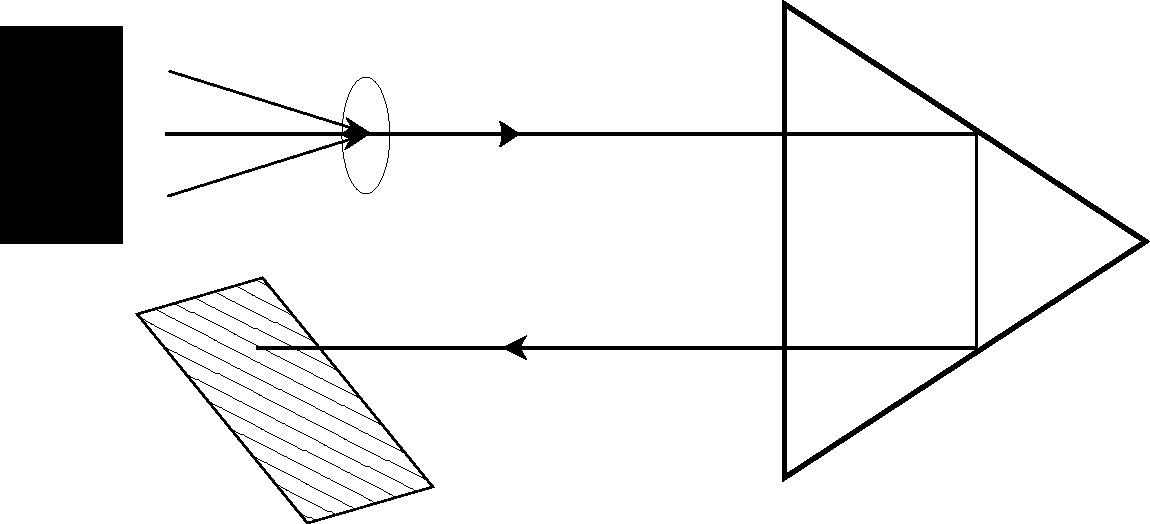
\includegraphics[height=5cm]{figures/linediagram.pdf}
%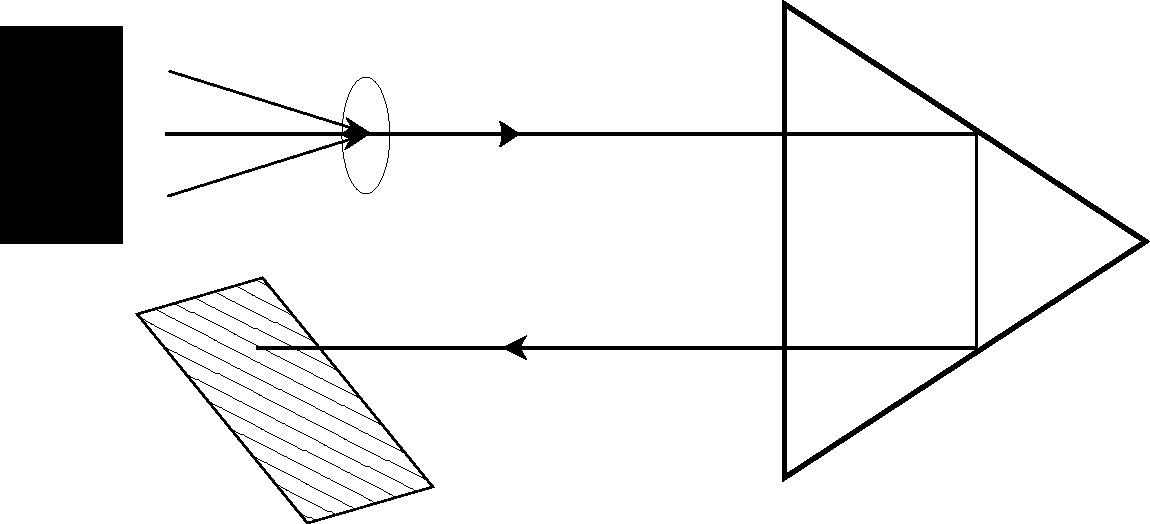
\includegraphics[height=5cm]{figures/linediagram.eps}
\caption{Tämä on esimerkki numeroidusta kuvatekstistä. \label{kuva1}}
\end{figure}

\begin{figure}[htb]
\centering
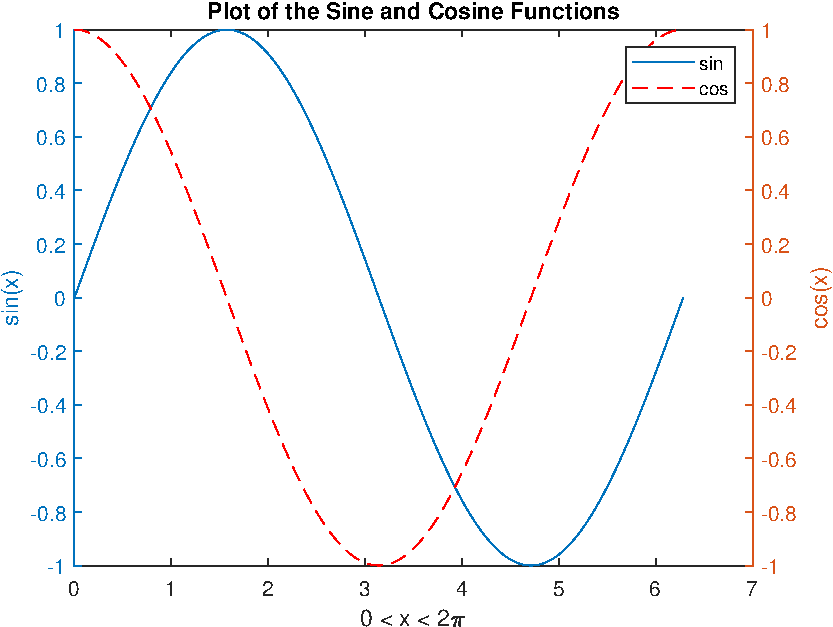
\includegraphics[height=5cm]{figures/curves.pdf}
%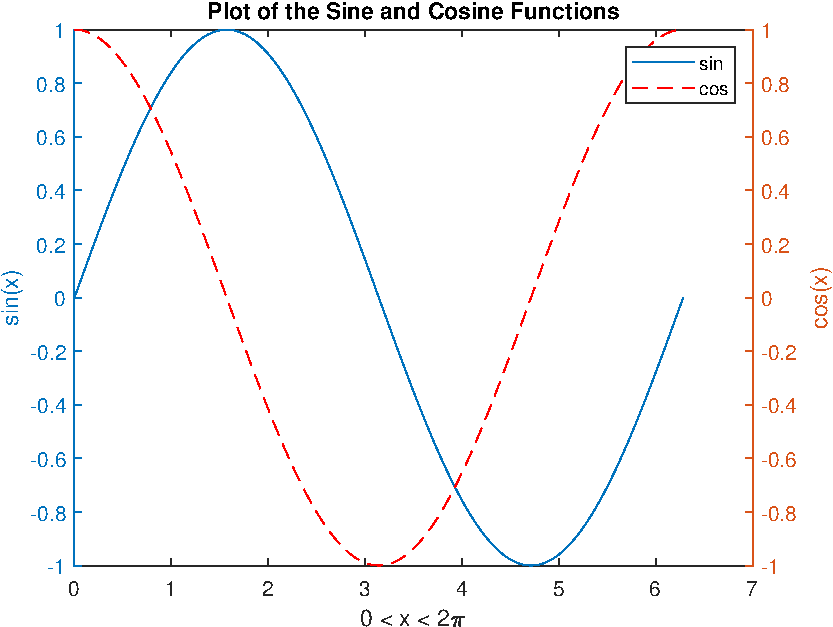
\includegraphics[height=5cm]{figures/curves.eps}
\caption{Tämä on esimerkki MATLAB-kuvasta. \label{kuva2}}
\end{figure}


\subsection{Lähdeviittausten käyttö} 

Lähdeviittaukset tulee tehdä huolellisesti ja johdonmukaisesti
numeroviitejärjestelmän mukaisesti. Numeroviitteet järjestetään
lähdeluetteloon viittausjärjestykseen, mutta jos lähdeluettelo
on hyvin laaja (useita sivuja), järjestetään viitteet pääsanan 
mukaiseen aakkosjärjestykseen. Alaviitejärjestelmää
\footnote{Myöskään alaviitteenä olevia kommentteja \underline{ei} suositella
käytettäviksi.} ei käytetä. 

Viitteen sijoittelussa noudatetaan seuraavia sääntöjä:
Jos viite kohdistuu vain yhteen virkkeeseen tai virkkeen 
osaan, viite \citep{Kauranen} sijoitetaan virkkeen sisään ennen virkettä
päättävää pistettä. Jos taas viite koskee tekstin useampaa
virkettä tai kokonaista kappaletta, sijoitetaan viite kappaleen loppuun 
pisteen jälkeen. \citep{Kauranen} 

Matematiikassa viitteet yleensä numeroidaan ja tekstissä lähteisiin viitataan numerolla (\emph{plain}-tyyli). Viitteet tulevat tällöin yleisimmin tekijän nimen mukaiseen aakkosjärjestykseen tai vaihtoehtoisesti siihen järjestykseen, jossa niihin viitataan.

\subsection{Lähdeluettelo} 

Lähdeluettelossa esiintyy tavallisesti seuraavassa esitettäviä
lähteitä, joista on numeroviitejärjestelmässä ilmoitettava
asianomaisessa kohdassa vaaditut tiedot.

%% Esimerkki korostamisesta. Lihavoinnin sijasta on tyylikkäämpää
%% ja luettavampaa käyttää kursiivia.
\textit{Kirjasta} ilmoitetaan seuraavat tiedot:

\begin{itemize}
\item[--]tekijät 
\item[--]julkaisun nimi
\item[--]painos, jos useita
\item[--]kustannuspaikka
\item[--]julkaisija tai kustantaja
\item[--]julkaisuaika
\item[--]mahdollinen sarjamerkintö. 
\end{itemize}

Viitteet \citep{Kauranen,Koblitz} ovat esimerkkejä kirjan
esittämisestä lähdeluettelossa. Viite \citep[s.\ 83--124]{Koblitz} on
esimerkki lähdeluettelossa esiintyvän kirjan tiettyjen sivujen
esittämisestä tekstissä.

\textit{Artikkelista} kausijulkaisussa ilmoitetaan seuraavat tiedot:

\begin{itemize}

\item[--]tekijät
\item[--]artikkelin nimi
\item[--]kausijulkaisun nimi
\item[--]julkaisuvuosi
\item[--]kausijulkaisun volyymi tai ilmestymisvuosi
\item[--]kausijulkaisun numero
\item[--]sivut, joilla artikkeli on.
\end{itemize}

\citet{bcs} ja \citet{Deschamps} ovat kirjoittaneet artikkelit, joita käytetään tässä esimerkkeinä artikkelin esittämisestä lähdeluettelossa.

\textit{Kokoomateoksen luvusta tai osasta} ilmoitetaan seuraavat tiedot:

\begin{itemize}
\item[--]luvun tai osan tekijät
\item[--]luvun tai osan nimi
\item[--]maininta >>Teoksessa>>
\item[--]koko teoksen toimittajat sekä maininta >>(toim.)>>
\item[--]koko teoksen tai konferenssin nimi
\item[--]konferenssiesitelmän kyseessä ollessa sen pitopaikka ja -aika
\item[--]painos, jos useita
\item[--]kustannuspaikka
\item[--]julkaisija tai kustantaja, jos aihetta tämän ilmoittamiseen on
\item[--]julkaisuaika
\item[--]sivut, joilla luku tai osa on 
\item[--]mahdollinen sarjamerkintä.
\end{itemize}

Viitteet \citep{Sihvola,Lindblom} ovat esimerkkejä
kokoomateoksen luvun tai osan esittämisestä lähdeluettelossa. 

\textit{Opinnäytetyöstä} ilmoitetaan seuraavat tiedot:

\begin{itemize}
\item[--]tekijä
\item[--]työn nimi
\item[--]opinnäytetyön tyyppi
\item[--]oppilaitoksen nimi
\item[--]oppilaitoksen sijaintipaikka
\item[--]vuosiluku.
\end{itemize}

Viitteet \citep{Miinusmaa,Lonnqvist} ovat esimerkkejä
opinnäytteen esittämisestä lähdeluettelossa. 


\textit{Haastattelusta} ilmoitetaan seuraavat tiedot:

\begin{itemize}
\item[--]haastatellun henkilön nimi
\item[--]haastatellun henkilön arvo tai asema
\item[--]haastatellun henkilön edustama organisaatio
\item[--]organisaation osoite
\item[--]maininta siitä, että kyseessä on haastattelu ja haastattelun
päivämäärä. 
\end{itemize}

Palmgrenin (\citeyear{haastattelu}) haastattelu on esimerkki
haastattelun esittämisestä lähdeluettelossa.

Osa sähköisessä muodossa olevista artikkeleista on saatavissa myös
painettuina. \textit{Vain verkosta saatavissa olevasta artikkelista} esitetään
seuraavat tiedot:

\begin{itemize}
\item[--]tekijät
\item[--]artikkelin nimi
\item[--]kausijulkaisun nimi
\item[--]viestintyyppi
\item[--]laitos tai volyymi
\item[--]kausijulkaisun yksittäistä osaa koskeva merkintä tai numero
\item[--]julkaisuvuosi tai maininta >>Päivitetty>> ja päivitysaika
\item[--]maininta >>Viitattu>> ja viittaamisen ajankohta 
\item[--]maininta >>Saatavissa>> ja URL tai 
        maininta >>DOI>> ja DOI-numero (DOI=Digital Object Identifier).
\end{itemize}

Viitteet \citep{Ribeiro,Stieber,kone} ovat esimerkkejä sähköisessä
muodossa olevan artikkelin esittämisestä opinnäytteen
lähdeluettelossa.  Viitteet \citep{Ribeiro} ja \citep{Stieber} ovat
saatavissa sekä painettuna että verkosta, joten viitteiden esitystapa
mukailee painetun artikkelin viitteen esitystapaa. Viite \citep{kone} on
saatavissa vain verkosta ja siitä esitetään yllä vaaditut tiedot.

Valitettavasti sähköisessä muodosssa olevasta artikkelista ei ole aina 
saatavissa lai\-tos-, volyymi- tai numerotietoja.

\textit{Sähköisessä muodossa olevasta opinnäytetyöstä} ilmoitetaan
seuraavat tiedot:
 
\begin{itemize}
\item[--]tekijä
\item[--]työn nimi
\item[--]opinnäytetyön tyyppi
\item[--]oppilaitoksen nimi
\item[--]oppilaitoksen sijaintipaikka
\item[--]vuosiluku

\end{itemize}

Viite \citep{Adida} on esimerkki sähköisessä muodossa olevan
opinnäytteen esittämisestä lähdeluettelossa.

Viite \citep{viittaaminen} on esimerkki itsenäisen kirjoituksen sisältävästä
verkkosivusta. Tällainen lähde on rinnastettavissa erillisteokseen.
\textit{Verkkosivusta} esitetään tiedot:

\begin{itemize}
\item[--] tekijät
\item[--] otsikko
\item[--] maininta "Päivitetty" ja päivitysaika 
\item[--] maininta "Viitattu" ja viittaamisen ajankohta
\item[--] Maininta "Saatavissa" ja URL.
\end{itemize}

Joskus verkkosivun kirjoitus on jaettu useammalle sivulle, jolloin
lähdeluetteloon kirjataan vain sellainen verkko-osoite, joka koskee
koko kirjoitusta tai sen etusivua, ellei sitten 
todella tarkoiteta kirjoituksen yksittäistä sivua. 

\subsection{Muuta huomioitavaa lähdeluettelossa}

%% Muutos vanhoihin ohjeisiin koskien kieltä.
Lähdeluettelossa työn ja julkaisun nimi kirjoitetaan alkuperäisessä
muodossaan. Julkaisijan kotipaikka kirjoitetaan alkukielisessä
muodossaan.

Viittamista koskevassa suomalaisessa standardissa
SFS 5342 \citep{sfs} vaaditaan julkaisuista ilmoitettavaksi myös ISBN- tai
ISSN-numerot, mutta näissä opinnäyteohjeissa ei ISBN- ja 
ISSN-numeroita vaadita. 